\chapter{Vector Integration}
\begin{enumerate}
	\item  If $\vec{F}=3 x y \hat{i}-y^{2} \hat{j}$ determine the value of $\int_{c} \vec{F} \cdot d \vec{r}$ where $C$ is the curve $y=2 x^{2}$ in the $x y$ plane from $(0,0)$ to $(1,2)$.
	\begin{figure}[H]
		\begin{center}
			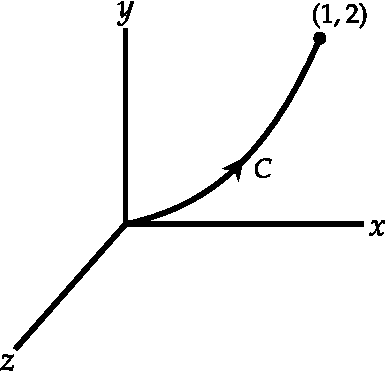
\includegraphics[width=4cm,height=4cm]{VI-Assignment-01}
		\end{center}
	\end{figure}
	\begin{answer}
		The curve lies in $x y$ plane, so, $z=0 . z$ can never be taken as independent variable $z$ is a dependent variable. Now, out of $x$ and $y$, any one variable can be taken as independent.
		Suppose $x$ is taken as independent variable
		\begin{align*}
		 y &=2 x^{2}, d y=4 x d x \\ \vec{F} \cdot d \vec{r} &=3 x y d x-y^{2} d y \\ &=6 x^{3} d x-4 x^{4} \cdot 4 x d x \\ &=\left(6 x^{3}-16 x^{5}\right) d x 
		 \intertext{So, the line integral $\int_{C} \vec{f} \cdot d \vec{r}$ reduces to a definite integral.}
		 \int_{0}^{1}\left(6 x^{3}-16 x^{5}\right) d x&\\
		 &=\left.6 \frac{x^{4}}{4}\right|_{0} ^{1}-\left.16 \frac{x^{6}}{6}\right|_{0} ^{1}\\
		 &=-\frac{7}{6}
		 \intertext{If $y$ is taken as independent variable then $x$ can be expressed in terms of $y$ as}
		 x &=\sqrt{\frac{y}{2}} \\ d x &=\frac{1}{2 \sqrt{2}} \frac{1}{\sqrt{y}} d y \\ \text{So}\quad \vec{f} \cdot d \vec{r} &=3 x y d x-y^{2} d y \\ &=3 y \sqrt{\frac{y}{2}} \cdot \frac{1}{2 \sqrt{2}} \frac{1}{\sqrt{y}} d y-y^{2} d y \\ &=\left(\frac{3}{4} y-y^{2}\right) d y 
		 \intertext{So, the line integral $\int \vec{f} . d \vec{r}$ reduces to a definite integral}
		 \int_{0}^{2}\left(\frac{3}{4} y-y^{2}\right) d y&\\
		 &=\frac{3}{8} y^{2}-\left.\frac{y^{3}}{3}\right|_{0} ^{2}\\
		 &=-\frac{7}{6}\\
		\end{align*}
	\end{answer}
	\item Evaluate $\int_{c} \vec{F} \cdot d \vec{r}$ where $\vec{F}=\left(x^{2}-y^{2}\right) \hat{i}+x y \hat{j}$ and curve $C$ is arc of the curve $y=x^{2}$ from $(0,0)$ to $(2,4)$
	\begin{answer}$\left. \right. $
		\begin{figure}[H]
			\centering
			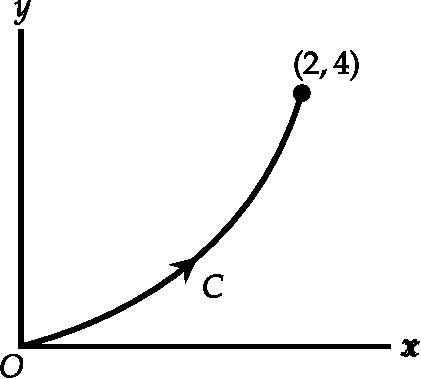
\includegraphics[height=3cm,width=3cm]{VI-Assignment-02}
		\end{figure}
		\begin{align*}
		\vec{F} \cdot d \vec{r}&=\left(x^{2}-y^{2}\right) d x+x y d y
	\intertext{	Taking $x$ as independent variable}
		y=x^{2} & d y=2 x d x \\
		\vec{F} \cdot d \vec{r} & =\left(x^{2}-y^{2}\right) d x+x y d y \\
		& =\left(x^{2}-x^{4}\right) d x+x^{3} \cdot 2 x d x \\
		& =\left(x^{2}+x^{4}\right) d x
		\intertext{So, the line integral $\int \vec{F} \cdot d \vec{r}$ reduces to a definite integral}
		\int_{0}^{2}\left(x^{2}+x^{4}\right) d x&=\frac{x^{3}}{3}+\left.\frac{x^{5}}{5}\right|_{0} ^{2}=\frac{136}{15}
		\intertext{Suppose a force acts on a particle and particles is displaced along a given path $C$. Then work done by the force $\vec{F}$ is given by line integral.}
		W&=\int_{C} \vec{F} \cdot d \vec{r}
		\intertext{The integration is being carried in the sense of displacement.}
		\end{align*}
	\end{answer}
	\item Find the work done when a force
	$$
	\vec{F}=\left(x^{2}-y^{2}+x\right) \hat{i}-(2 x y+y) \hat{j}
	$$
	moves a particle in $x y$ plane from $(0,0)$ to $(1,1)$ along the parabola $y^{2}=x$
	\begin{answer}$\left. \right. $
		\begin{figure}[H]
			\centering
			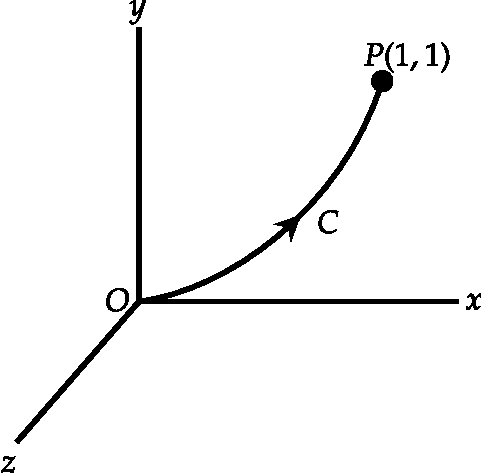
\includegraphics[height=3.5cm,width=3.5cm]{VI-Assignment-03}
		\end{figure}
		\begin{align*}
		\intertext{Here, on the curve $C, y$ can be taken as independent variable and}
	x&=y^{2}, d x=2 y d y
	\intertext{workdone in moving a particle by displacement $d \vec{r}$}
	d W &=\vec{F} \cdot d \vec{r} \\ &=\left(x^{2}-y^{2}+x\right) d x-(2 x y+y) d y \\ &=\left(y^{4}-y^{2}+y^{2}\right) \cdot 2 y d y-\left(2 y^{2} \cdot y+y\right) d y \\ &=\left(2 y^{5}-2 y^{3}-y\right) d y 
	\intertext{Hence, work done is moving a particle from $O$ to $P$ is given by}
	W&=\int_{0}^{1}\left(2 y^{5}-2 y^{3}-y\right) d y=2 \frac{y^{6}}{6}-2 \frac{y^{4}}{4}-\left.\frac{y^{2}}{2}\right|_{0} ^{1}=-\frac{2}{3}
		\end{align*}
	\end{answer}
	\item Evaluate $\oint x d y-y d x$ around a circle $x^{2}+y^{2}=r^{2}$
	\begin{answer}$\left. \right. $
		\begin{figure}[H]
			\centering
			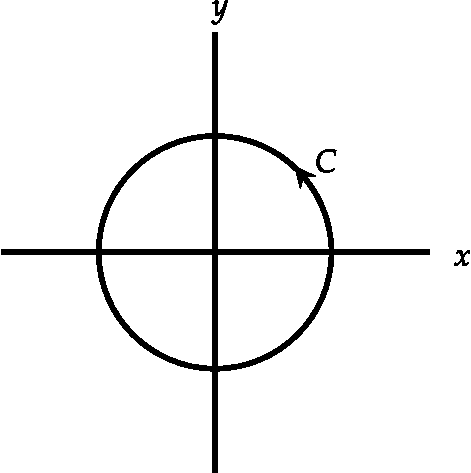
\includegraphics[height=4cm,width=4cm]{VI-Assignment-04}
		\end{figure}
		\begin{align*}
	\intertext{	Let $C$ denotes the circle. The parametric equations of circle is}
		&x=r \cos \theta \\
		&y=r \sin \theta
		\intertext{Here, $x$ and $y$ have been expressed in terms of parameter which varies from 0 to $2 \pi$ as one traverses the circle.}
		x&=r \cos \theta \Rightarrow d x=-r \sin \theta d \theta\\
		y&=r \sin \theta \Rightarrow d y=r \cos \theta d \theta\\
		 x d y-y d x &=r \cos \theta r \cos \theta d \theta-r \sin \theta(-r \sin \theta) d \theta \\ &=r^{2} d \theta \\
		\text{ So,}\quad
		 \oint_{c} x d y-y d x&=r^{2} \oint d \theta \\
		 &=2 \pi r^{2}
		 \intertext{Here, $r$ is a constant, because integral is carried over a circle.}
		\end{align*}
	\end{answer}
	\item  Calculate the work done when a force $\vec{F}=x y \hat{i}+\left(x^{2}+y^{2}\right) \hat{j}$ moves a particle in $x y$ plane from $(1,0)$ to $(3,8)$ along the curve $C, y=x^{2}-1$.
	\begin{answer}$\left. \right. $
		\begin{figure}[H]
			\centering
			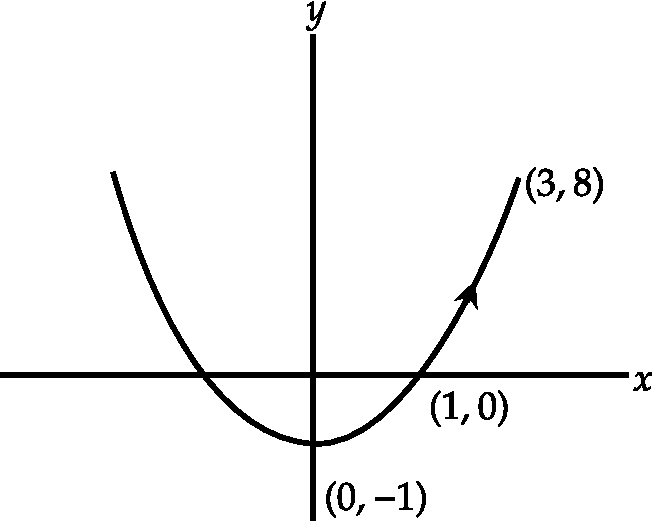
\includegraphics[height=4cm,width=5cm]{VI-Assignment-05}
		\end{figure}
		The curve $C$ is $y=x^{2}-1$. Since, this is quadratic in $x$ and linear in $y$ with no $x y$ terms. This is a parabola. Let us put this parabola in the form
		\begin{align*}
		(x-\alpha)^{2} &=4 a(y-\beta) \\ C:(x-0)^{2} &=(y+1) 
		\intertext{This is a parabola with vertex at $(0,-1)$ and axis parallel to $y$ axis.}
		\intertext{On curve $C$, let us take $x$ as indepedent variable. The dependent variable $y$ can be written in terms of $x$ as}
		 y &=x^{2}-1 \\ d y &=2 x d x 
		 \intertext{work done is moving a particle by displacement $d \vec{r}$}
		  d W &=\vec{F} \cdot d \vec{r} \\ &=x y d x+\left(x^{2}+y^{2}\right) d y \\ &=x\left(x^{2}-1\right) d x+\left(x^{2}+\left(x^{2}-1\right)^{2}\right) 2 x d x \\ &=\left(2 x^{5}-x^{3}+x\right) d x 
		  \intertext{So, work done is moving a particle from $(1,0)$ to $(3,8)$ along a curve $C$.}
		   W &=\int_{c} \vec{F} \cdot d \vec{r}=\int_{1}^{3}\left(2 x^{5}-x^{3}+x\right) d x \\ &=\left.\left(2 \cdot \frac{x^{6}}{6}-\frac{x^{4}}{4}+\frac{x^{2}}{2}\right)\right|_{1} ^{3}=227 
		\end{align*}
	\end{answer}
	\item Evaluate the line integral $\int_{c} \vec{F} \cdot d \vec{r}$ where $\vec{F}=(x+2 y) \hat{i}+(2 y-x) \hat{j}$ and $C$ is curve in $x y$ plane consisting of the straight lines from $(0,0)$ to $(1,0)$ and then to $(3,4)$.
	\begin{answer}
		The curve $C$ consists of two pieces of smooth curves $C_{1}$ and\\ $C_{2}$. $C_{1}$ is straight line from $(0,0)$ to $(1,0)$ ie. $y=0$\\
		$C_{2}$ is straight line from $(1,0)$ to $(3,4)$
		\begin{figure}[H]
			\centering
			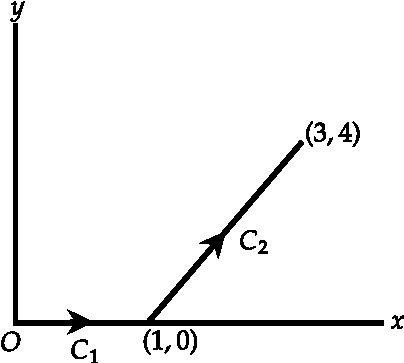
\includegraphics[height=3.5cm,width=3.5cm]{VI-Assignment-06}
		\end{figure}
		\begin{align*}
		\text{i.e}.\qquad \quad y-0&=\left(\frac{4-0}{3-1}\right) \cdot(x-1)\\
		\text{or, }\qquad y&=2 x-2\\
		\text{So, along }C_{1}, y&=0, d y=0 \text{( $x$ is an independent variable )}\\
		\vec{F} \cdot d \vec{r}&=x d x\\
	\text{	Along }C_{2} ; y&=2 x-2, d y=2 d x\text{ (let us take $x$ as independent variables).}\\
		\vec{F} \cdot d \vec{r}&=(x+2 y) d x+(2 y-x) d y\\
	\text{	on }\quad C_{2}, \quad \vec{F} \cdot d \vec{r} &=(x+2(2 x-2)) d x+(2(2 x-2)-x) \cdot 2 d x \\ &=(11 x-12) d x \\
	\text{So,}\quad
	\int_{c} \vec{F} \cdot d \vec{r}&=\int_{c_{1}} \vec{F} \cdot d \vec{r}+\int_{C_{2}} \vec{F} \cdot d \vec{r}\\
	&=\int_{0}^{1} x d x+\int_{1}^{3}(11 x-12) d x\\
	&=\left.\frac{x^{2}}{2}\right|_{0} ^{1}+\left.\left(\frac{11}{2} x^{2}-12 x\right)\right|_{1} ^{3}\\
	&=20.5
		\end{align*}
	\end{answer}
	\item Evaluate $\oint_{C} \vec{F} \cdot d \vec{r}$ where $\vec{F}=\left(x^{2}+y^{2}\right) \hat{i}-2 x y \hat{j}$, where curve $C$ is a rectangle in the $x y$ plane bounded by $y=0, x=a, y=b, x=0$.
	\begin{answer}$\left. \right. $
			\begin{figure}[H]
			\centering
			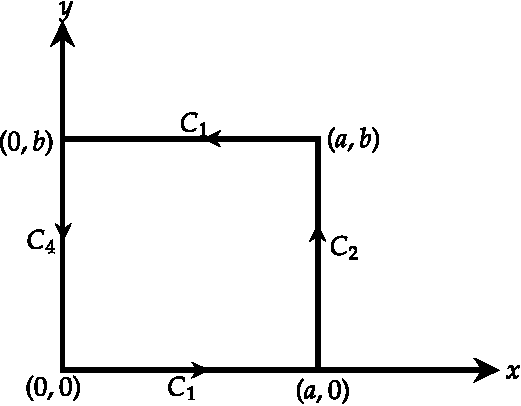
\includegraphics[height=4cm,width=4.6cm]{VI-Assignment-07}
		\end{figure}
		\begin{align*}
		\intertext{The curve $C$ as shown in figure $8.11$ consists of four pieces of smooth curves $C_{1}, C_{2}, C_{3} \& C_{4}$. }
		\vec{F} \cdot d \vec{r}&=\left(x^{2}+y^{2}\right) d x-2 x y d y\\
		\text{On }C_{1}, y&=0, d y=0, \vec{F} . d \vec{r}=x^{2} d x\\
	\text{	On }C_{2}, x&=a, d x=0, \vec{F} \cdot d \vec{r}=-2 a y d y\\
		\text{On }C_{3}, y&=b, d y=0, \vec{F} \cdot d \vec{r}=\left(x^{2}+b^{2}\right) d x\\
		\text{On }C_{4}, x&=0, d x=0, \vec{F} . d \vec{r}=0\\
		\oint \vec{F} \cdot d \vec{r}&=\int_{C_{1}} \vec{F} \cdot d \vec{r}+\int_{C_{2}} \vec{F} \cdot d \vec{r}+\int_{C_{3}} \vec{F} \cdot d \vec{r}+\int_{C_{4}} \vec{F} \cdot d \vec{r}\\
		&=\int_{0}^{a} x^{2} d x+\int_{0}^{b}-2 a y d y+\int_{a}^{0}\left(x^{2}+b^{2}\right) d x+\int_{b}^{0} 0 . d y\\
		&=\left.\frac{x^{3}}{3}\right|_{0} ^{a}+\left[-a y^{2}\right]_{0}^{b}+\left[\frac{x^{3}}{3}+b^{2} x\right]_{a}^{0}\\
		&=\frac{a^{3}}{3}-a b^{2}-\frac{a^{3}}{3}-a b^{2}\\
		&=-2 a b^{2}
		\end{align*}
	\end{answer}
	\item Find the total work done in moving a particles in a force field given by $\vec{F}=3 x y \hat{i}-5 z \hat{j}+10 x \hat{k}$ along the curve $x=t^{2}+1, y=2 t^{2}, z=t^{3}$ from $t=1$ to $t=2$.
	\begin{answer}
		\begin{align*}
		\intertext{On curve $C$, the coordinates $x, y, z$ are expressed in terms of parameter $t$.}
		&x=t^{2}+1, d x=2 t d t \\
		&y=2 t^{2}, d y=4 t d t \\
		&z=t^{3}, d z=3 t^{2} d t\\
		t\text{ varies from }t&=1\text{ to }t=2.\\
		 \vec{F} \cdot d \vec{r} &=3 x y d x-5 z d y+10 x d z \\ &=3\left(t^{2}+1\right) \cdot 2 t^{2} \cdot 2 t d t-5 t^{3} 4 t d t+10\left(t^{2}+1\right) \cdot 3 t^{2} d t \\ &=\left(12 t^{5}+10 t^{4}+12 t^{3}+30 t^{2}\right) d t \\
		 \text{So, total}&\text{ work done,}\\
		  W &=\int_{C} \vec{F} \cdot d \vec{r} \\ &=\int_{1}^{2}\left(12 t^{5}+10 t^{4}+12 t^{3}+30 t^{2}\right) d t \\ &=\left.\left(12 \frac{t^{6}}{6}+10 \frac{t^{5}}{5}+12 \frac{t^{4}}{4}+30 \frac{t^{3}}{3}\right)\right|_{1} ^{2} \\ &=303 
		\end{align*}
	\end{answer}
	\item 
	Find the work done in moving a particle once around a circle $C$ in the $x y$ plane if the circle has a centre at the origin and radius 2 and if the force field $\vec{F}$ is given by
	$$\vec{F}=(2 x-y+2 z) \hat{i}+(x+y-z) \hat{j}+(3 x-2 y-5 z) \hat{k}$$
	\begin{answer}	Equation of circle as shown in figure $8.12$ is written in parametric form as
		\begin{figure}[H]
			\centering
			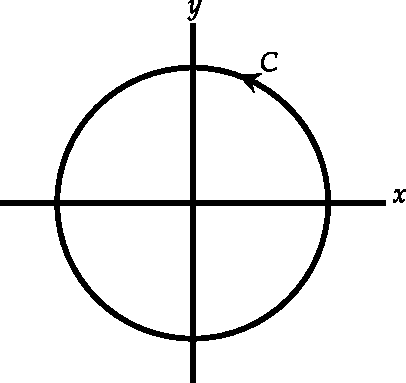
\includegraphics[height=3.8cm,width=4cm]{VI-Assignment-08}
		\end{figure}
		\begin{align*}
		x&=2 \cos \theta \Rightarrow d x=-2 \sin \theta d \theta\\
		y&=2 \sin \theta  \Rightarrow d y=2 \cos \theta d \theta \\ z&=0  \Rightarrow d z=0
		\intertext{$x, y, z$ are expressed in terms of parameter $\theta$.}
	 \vec{F} \cdot d \vec{r}=&(2 x-y+2 z) d x+(x+y-z) d y+(3 x-2 y-5 z) d z \\=&(4 \cos \theta-2 \sin \theta)(-2 \sin \theta) d \theta \\ & \quad+(2 \cos \theta+2 \sin \theta)(6 \cos \theta-4 \sin \theta) .0 \\=&(4-4 \sin \theta \cos \theta) d \theta \\
	 \text{$\theta$ varies from 0 to $2 \pi$}&\\
	 \text{So, total work done}&\\
	  W &=\int_{0}^{2 \pi}(4-4 \sin \theta \cos \theta) d \theta \\ &=4 \theta-\left.2 \sin ^{2} \theta\right|_{0} ^{2 \pi} \\ &=8 \pi 
		\end{align*}
	\end{answer}
	\item If $\vec{F}=\left(3 x^{2}+6 y\right) \hat{i}-14 y z \hat{j}+20 x z^{2} \hat{k}$. Evaluate $\int \vec{F} \cdot d \vec{r}$ where $C$ is a straight line joining $(0,0,0)$ to $(1,1,1)$.
	\begin{answer}
		Equation of straight line joining $(0,0,0)$ to $(1,1,1)$ is given by $\frac{x-0}{1-0}=\frac{y-0}{1-0}=\frac{z-0}{1-0}=t$, where $t$ is parameter.
		\begin{align*}
		\intertext{In parametric form, equation of curve is given by}
		x&=t \Rightarrow d x=d t\\
		y&=t \Rightarrow d y=d t\\
		z&=t \Rightarrow d z=d t
		\intertext{$t$ varies from 0 to 1 .}
		 \vec{F} \cdot d \vec{r} &=\left(3 x^{2}+6 y\right) d x-14 y z d y+20 x z^{2} d z \\ &=\left(20 t^{3}-11 t^{2}+6 t\right) d t \\ \int_{C} \vec{F} \cdot d \vec{r} &=\int_{0}^{1}\left(20 t^{3}-11 t^{2}+6 t\right) d t \\ &=\left.\left(5 t^{4}-\frac{11}{3} t^{3}+3 t^{2}\right)\right|_{0} ^{1} \\ &=\frac{13}{3} 
		\end{align*}
	\end{answer}
	\item  Integrate the function $\vec{F}=x^{2} \hat{i}-x y \hat{j}$ from the point $(0,0)$ to $(1,1)$ along the parabola $y^{2}=x$.
	\begin{answer}
		Here the curve $C$ is parabola $y^{2}=x$ as shown in figure 8.13. On $C, y$ can be taken as independent variable.
		\begin{figure}[H]
			\centering
			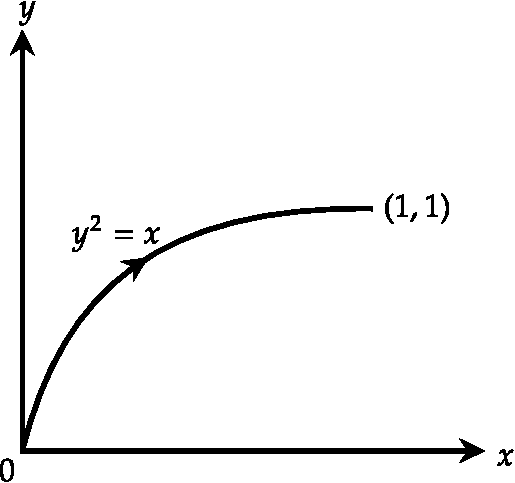
\includegraphics[height=4cm,width=4cm]{VI-Assignment-09}
		\end{figure}
		\begin{align*}
		\intertext{The dependent variable $x$ can be written in terms of $y$ as}
		x&=y^{2}\\
		d x&=2 y d y\\
		 \vec{F} \cdot d \vec{r} &=x^{2} d x-x y d y \\ &=y^{4} \cdot 2 y d y-y^{2} \cdot y d y \\ &=\left(2 y^{5}-y^{3}\right) d y 
		 \text{So, the line integral}\\
		 \int_{C} \vec{F} \cdot d \vec{r} &=\int_{0}^{1}\left(2 y^{5}-y^{3}\right) d y \\ &=\frac{1}{3} y^{6}-\left.\frac{1}{4} y^{4}\right|_{0} ^{1}=\frac{1}{12} 
		\end{align*}
	\end{answer}
\item Find the value of $\int_{C}\left[\left(x+y^{2}\right) d x+\left(x^{2}-y\right) d y\right]$ taken in the counter-clockwise sense along the closed curve $C$ formed by $y^{3}=x^{2}$ and the straight line $y=x$.
\begin{answer}
	The curve $C$ consists of chord $O A$ and curved part $A O$ as shown in figure 8.14.\\
	Equation of $O A$ is $y=x$ and curved part is $y^{3}=x^{2}$.\\
	Along chord $O A, x$ can be taken as independent variable and $y=x$.
	\begin{figure}[H]
		\centering
		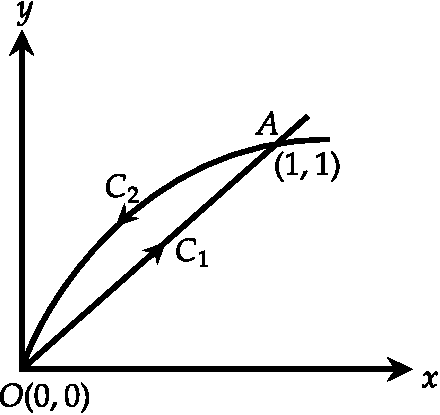
\includegraphics[height=4cm,width=4cm]{VI-Assignment-10}
	\end{figure}
	\begin{align*}
	 \vec{F} \cdot d \vec{r} &=\left(x+y^{2}\right) d x+\left(x^{2}-y\right) d y \\ &=\left(x+x^{2}\right) d x+\left(x^{2}-x\right) d x \\ &=2 x^{2} d x 
	 \intertext{Along $O A, x$ varies from 0 to 1 . On curved part $A O$, let $y$ be taken as independent variable $\&$ dependent variable $x$ can be put as}
	 x&=y^{3 / 2}, d x=\frac{3}{2} y^{1 / 2} d y\\
	  \vec{F} \cdot d \vec{r} &=\left(x+y^{2}\right) d x+\left(x^{2}-y\right) d y \\ &=\left(y^{3 / 2}+y^{2}\right) \frac{3}{2} y^{1 / 2} d y+\left(y^{3}-y\right) d y \\ &=\left(y^{3}+\frac{3}{2} y^{5 / 2}+\frac{3}{2} y^{2}-y\right) d y \\
	  \text{$y$ varies from 1 to $0 .$}\\
	  \oint_{C} \vec{F} \cdot d \vec{r}&=\int_{C_{1}} \vec{F} \cdot d \vec{r}+\int_{C_{2}} \vec{F} \cdot d \vec{r}\\
	  &=\int_{0}^{1} 2 x^{2} d x+\int_{1}^{0}\left(y^{3}+\frac{3}{2} y^{5 / 2}+\frac{3}{2} y^{2}-y\right) d y\\
	  &=\left.\frac{2}{3} x^{3}\right|_{0} ^{1}+\frac{1}{4} y^{4}+\frac{3}{7} y^{7 / 2}+\frac{1}{2} y^{3}-\left.\frac{1}{2} y^{2}\right|_{1} ^{0}\\
	  &=-\frac{1}{84}
	  \intertext{
	  	Note:- If the integral is carried out in clockwise direction. The answer will differ only in sign. $\oint_{C} \vec{F} \cdot d \vec{r}$ in clockwise direction $=\frac{1}{84}$}
	\end{align*}
\end{answer}
\item Calculate $\int_{C} \vec{F} \cdot d \vec{r}$ where $\vec{F}=\frac{y^{2}}{x^{2}+y^{2}} \hat{i}-\frac{x^{2}}{x^{2}+y^{2}} \hat{j}$, where $C$ is the semi-circle $y=\sqrt{a^{2}-x^{2}}$.
\begin{answer}$\left. \right. $
	\begin{figure}[H]
		\centering
		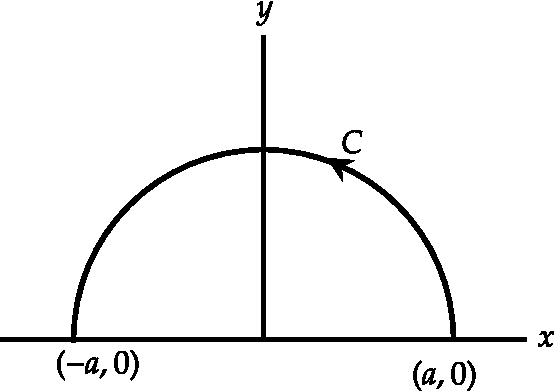
\includegraphics[height=3.5cm,width=5cm]{VI-Assignment-11}
	\end{figure}
	The curve $C$ shown in Figure $8.15$ is the semi-circle
	\begin{align*}
	y&=\sqrt{a^{2}-x^{2}}
	\intertext{The equation can be written in parametric form as}
	x&=a \cos \theta \Rightarrow d x=-a \sin \theta d \theta\\
	y&=a \sin \theta \Rightarrow d y=a \cos \theta d \theta
	\intertext{$\theta$ varies from 0 to $\pi$.}
	\vec{F} \cdot d \vec{r}&=\frac{y^{2} d x-x^{2} d y}{x^{2}+y^{2}}\\
	&=\frac{a^{2} \sin ^{2} \theta(-a \sin \theta) d \theta-\left(a^{2} \cos ^{2} \theta\right) a \cos \theta d \theta}{a^{2}}\\
	&=-a\left(\sin ^{3} \theta+\cos ^{3} \theta\right) d \theta\\
	\int_{C} \vec{F} \cdot d \vec{r}&=-a \int_{0}^{\pi}\left(\sin ^{3} \theta+\cos ^{3} \theta\right) d \theta\\
	&=-a \int_{0}^{\pi} \sin ^{3} \theta d \theta-a \int_{0}^{\pi} \cos ^{3} \theta d \theta\\
	&=-2 a \int_{0}^{\pi / 2} \sin ^{3} \theta d \theta-0\left(\right.
	\text{ Since, }\left.\int_{0}^{\pi} \cos ^{3} \theta d \theta=0\right)\\
	&=-2 a \frac{\sqrt{2} \sqrt{1 / 2}}{2 \cdot \sqrt{5 / 2}}\\
	&=-\frac{4 a}{3}
	\end{align*}
\end{answer}
\item Evaluate $\int_{C} \frac{d x}{x+y}$ where $C$ is the curve $y^{2}=4 a x$ from $(0,0)$ to $(4 a, 4 a)$.
\begin{answer}
	The equation of curve (as shown in the figure 8.16) can be written in parametric form as
	\begin{figure}[H]
		\centering
		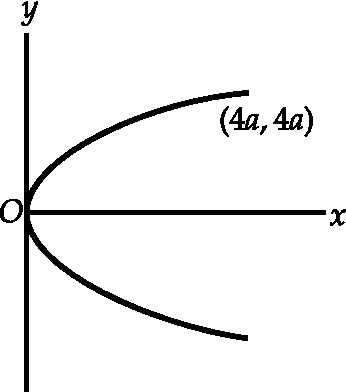
\includegraphics[height=3.7cm,width=3.5cm]{VI-Assignment-12}
	\end{figure}
	\begin{align*}
	x&=a t^{2} \Rightarrow d x=2 a t d t\\
	y&=2 a t \Rightarrow d y=2 a d t
	\intertext{Parameter, $t$ varies from 0 to 2 .}\\
	\text{The integral}\\
	 \int_{0} \frac{d x}{x+y} &=\int_{0}^{2} \frac{2 a t d t}{a t^{2}+2 a t}=2 \int_{0}^{2} \frac{d t}{t+2}=\left.2 \log (t+2)\right|_{0} ^{2} \\ &=2 \log 2 
	\end{align*}
\end{answer}
\item Evaluate $\int_{C}(y d x-x d y)$, where $C$ is arc of cycloid $x=2(\theta-\sin \theta), y=2(1-\cos \theta)$ joining the points $(0,0)$ and $(4 \pi, 0)$.
\begin{answer}
		The parametric equation of curve $C$ as shown in figure $8.17$ is given as
		\begin{figure}[H]
			\centering
			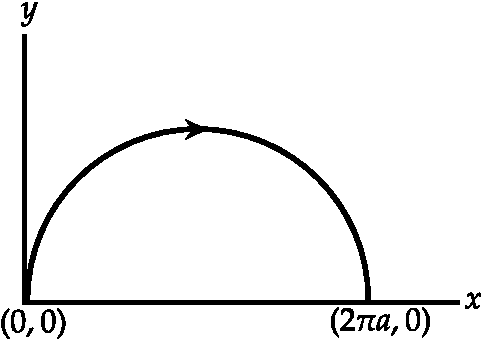
\includegraphics[height=3.5cm,width=5cm]{VI-Assignment-13}
		\end{figure}
	\begin{align*}
	x&=2(\theta-\sin \theta) \Rightarrow d x=2(1-\cos \theta) d \theta \\
	y&=2(1-\cos \theta) \Rightarrow d y=2 \sin \theta d \theta
	\intertext{$\theta$ is the parameter since $(x, y)$ varies from $(0,0)$ to $(4 \pi, 0)$. So, $\theta$ will vary from 0 to $2 \pi$.
		The integrand $y d x-x d y$}
	&=2(1-\cos \theta) \cdot 2(1-\cos \theta) d \theta-2(\theta-\sin \theta) \cdot 2 \sin \theta d \theta\\
	&=4(2-2 \cos \theta-\theta \sin \theta)\\
\text{	So,}\quad
	\int_{C} y d x-x d y&=4 \int_{0}^{2 \pi}(2-2 \cos \theta-\theta \sin \theta) d \theta\\
	&=8 \int_{0}^{2 \pi} d \theta-8 \int_{0}^{2 \pi} \cos \theta d \theta-4 \int_{0}^{2 \pi} \theta \sin \theta d \theta\\
	&=16 \pi-8[\sin \theta]_{0}^{2 \pi}-4[-\theta \cos \theta+\sin \theta]_{0}^{2 \pi}\\
	&=24 \pi
	\end{align*}
\end{answer}
\item Evaluate $\int_{C} \vec{F} \cdot d \vec{r}$ where $\vec{F}=(2 a-y) \hat{i}-(a-y) \hat{j}$ where $C$ is the arc of the cycloid $x=a(\theta-\sin \theta)$, $y=a(1-\cos \theta)$ from $(0,0)$ to $(2 \pi a, 0)$.
\begin{answer}
	The equation of cycloid is written in parametric form as
	\begin{align*}
	x&=a(\theta-\sin \theta) \Rightarrow d x=a(1-\cos \theta) d \theta\\
	y&=a(1-\cos \theta) \Rightarrow d y=a \sin \theta d \theta
	\intertext{where $\theta$ is the parameter varying from 0 to $2 \pi$.}
\text{	On $C:$}
	\vec{F} \cdot d \vec{r} &=(2 a-y) d x-(a-y) d y \\
	&=a(1+\cos \theta) \cdot a(1-\cos \theta) d \theta-a \cos \theta \cdot a \sin \theta d \theta \\
	&=a^{2}\left(1-\cos ^{2} \theta-\sin \theta \cos \theta\right) d \theta
	\intertext{So, the line integral}
	 \int_{C} \vec{F} \cdot d \vec{r} &=a^{2} \int_{0}^{2 \pi}\left(1-\cos ^{2} \theta-\sin \theta \cos \theta\right) d \theta \\ &=a^{2} \int_{0}^{2 \pi} d \theta-a^{2} \int_{0}^{2 \pi} \cos ^{2} \theta d \theta-a^{2} \int_{0}^{2 \pi} \sin \theta \cos \theta d \theta \\ &=\pi a^{2} 
	\end{align*}
\end{answer}
\item Evaluate $\int_{C} \frac{x^{2} d y-y^{2} d x}{x^{5 / 3}+y^{5 / 3}}$
where $C$ is the quarter of the astroid $x=a \cos ^{3} t, y=a \sin ^{3} t$ from the point $(a, 0)$ to the point $(0, a)$.
\begin{answer}
	The parametric equation of the astroid as shown in figure $8.18$ is given as
	\begin{figure}[H]
		\centering
		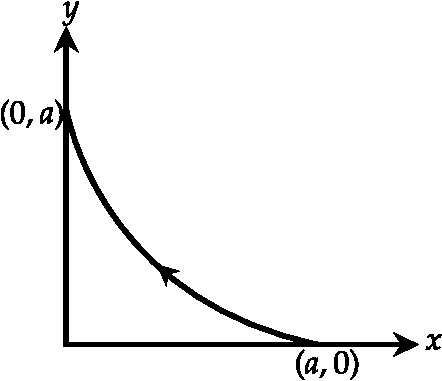
\includegraphics[height=3.5cm,width=4cm]{VI-Assignment-14}
	\end{figure}
	\begin{align*}
	x&=a \cos ^{3} t \Rightarrow d x=-3 a \cos ^{2} t \sin t d t\\
	y&=a \sin ^{3} t \Rightarrow d y=3 a \sin ^{2} t \cos t d t
	\intertext{$(x, y)$ varies from $(a, 0)$ to $(0, a)$.}
	\intertext{So, $t$ varies from 0 to $\pi / 2$.}
	\text{The integrand }&\frac{x^{2} d y-y^{2} d x}{x^{5 / 3}+y^{5 / 3}}\\
	&=\frac{a^{2} \cos ^{6} t\left(3 a \sin ^{2} t \cos t\right) d t-\left(a^{2} \sin ^{6} t\right) \cdot\left(-3 a \cos ^{2} t \sin t\right) d t}{a^{5 / 3}\left(\cos ^{5} t+\sin ^{5} t\right)}\\
	&=3 a^{4 / 3} \sin ^{2} t \cos ^{2} t d t
	\intertext{The line integral reduces to}
	3 a^{4 / 3} \int_{0}^{\pi / 2} \sin ^{2} t \cos ^{2} t d t&=3 a^{4 / 3} \frac{\sqrt{3 / 2 / 3 / 2}}{2 \sqrt{3}}=\frac{3 \pi a^{4 / 3}}{16}
	\end{align*}
\end{answer}
\item Find the value of $\int_{c}\left(x^{2}+y^{2}\right) d y$ taken in the counter clockwise sense along the quadrilateral with vertices $(0,0),(2,0),(4,4),(0,4)$.
\begin{answer}
	The quadirlateral as shown in Figure $8.19$ consists of four pieces of smooth curves $A B, B C, C D $\&$ D A$.
	\begin{figure}[H]
		\centering
		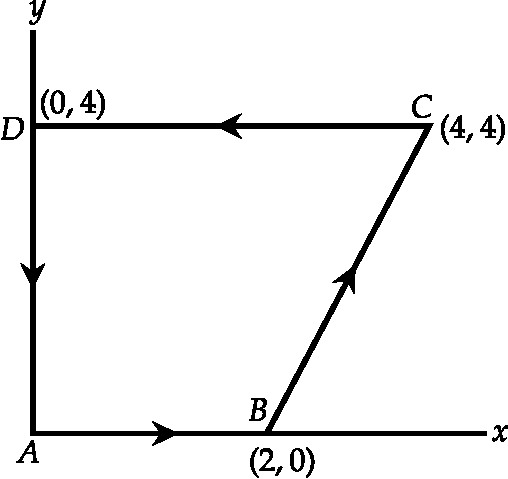
\includegraphics[height=4cm,width=4cm]{VI-Assignment-15}
	\end{figure}
	\begin{align*}
	\text{On }A B, y&=0, d y=0,\left(x^{2}+y^{2}\right) d y=0\\
	 y &=2 x-4, d y=2 d x \\\left(x^{2}+y^{2}\right) d y &=\left(x^{2}+(2 x-4)^{2}\right) 2 d x \\ &=\left(10 x^{2}-32 x+32\right) d x \\
	 \text{$x$ varies from 2 to 4}\\
	 \text{On CD, }y&=4, d y=0\\
	 \left(x^{2}+y^{2}\right) d y=0\\
	 \text { On  D A, }x&=0, d x=0\\
	 \left(x^{2}+y^{2}\right) d y&=y^{2} d y\\
	 \text{$y$ varies from 4 to 0}\\
	\text{ So, the line integral}\\
	 \int_{C}\left(x^{2}+y^{2}\right) d y &=\int_{A B}\left(x^{2}+y^{2}\right) d y+\int_{B C}\left(x^{2}+y^{2}\right) d y+\int_{C D}\left(x^{2}+y^{2}\right) d y+\int_{D A}\left(x^{2}+y^{2}\right) d y \\ &=0+\int_{2}^{4}\left(10 x^{2}-32 x+32\right) d x+0+\int_{4}^{0} y^{2} d y \\ &=\left.\left(\frac{10}{3} x^{3}-16 x^{2}+32 x\right)\right|_{2} ^{4}+\left.\frac{y^{3}}{3}\right|_{4} ^{0} \\ &=\frac{112}{3} 
	\end{align*}
\end{answer}
\item  Evaluate $\int_{C} x y^{2} d y-x^{2} y d x$ taken in the counter clockwise sense along the cardioid $r=a(1+\cos \theta)$
\begin{answer}
	The curve $C$ as shown in figure $8.20$ cardiod whose equation is
	\begin{figure}[H]
		\centering
		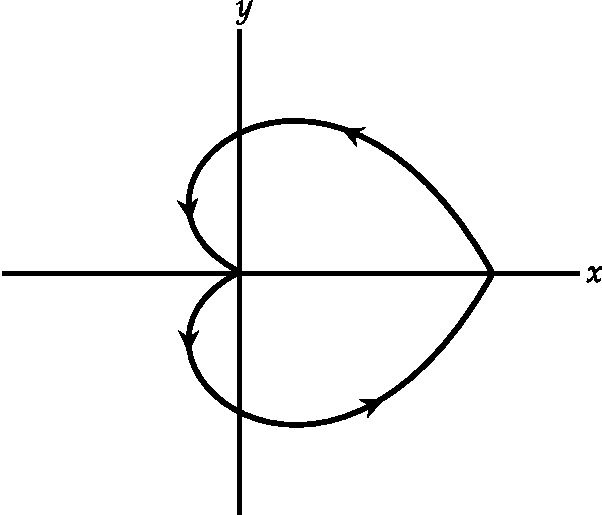
\includegraphics[height=4cm,width=5cm]{VI-Assignment-16}
	\end{figure}
	\begin{align*}
	r&=a(1+\cos \theta)\\
	x&=r \cos \theta=a(1+\cos \theta) \cos \theta=a\left(\cos \theta+\cos ^{2} \theta\right)\\
	d x&=a(-\sin \theta-2 \cos \theta \sin \theta) d \theta\\
	y &=r \sin \theta=a(1+\cos \theta) \sin \theta=a(\sin \theta+\sin \theta \cos \theta) \\ d y &=a\left(\cos \theta+\cos ^{2} \theta-\sin ^{2} \theta\right) d \theta \\
	\text{The integrand}&\\
	\left(x y^{2} d y-x^{2} y d x\right)&\\
	&=r^{3} \cos \theta \sin ^{2} \theta a\left(\cos \theta+\cos ^{2} \theta-\sin ^{2} \theta\right) d \theta\\
	&\quad \quad-r^{3} \cos ^{2} \theta \sin \theta a(\sin \theta-2 \cos \theta \sin \theta) d \theta\\
	&=a r^{2} \cos \theta \sin ^{2} \theta\left(\cos \theta+\cos ^{2} \theta-\sin ^{2} \theta+\cos \theta+2 \cos ^{2} \theta\right) d \theta\\
	&=a^{4}(1+\cos \theta)^{3} \cos \theta \sin ^{2} \theta\left(4 \cos ^{2} \theta+2 \cos \theta-1\right) d \theta\\
	&=a^{4}\left[\cos ^{6} \theta \sin ^{2} \theta+14 \cos ^{5} \theta \sin ^{2} \theta+17 \cos ^{4} \theta \sin ^{2} \theta\right.\\
	&\left.\quad+7 \cos ^{3} \theta \sin ^{2} \theta-\cos ^{2} \theta \sin ^{2} \theta-\cos \theta \sin ^{2} \theta\right]\\
	\text{The line integral}&\\
	\oint\left(x y^{2} d y-x^{2} y d x\right)&\\
	&=a^{4} \int_{0}^{2 \pi}\left(\cos ^{6} \theta \sin ^{2} \theta+14 \cos ^{5} \theta \sin ^{2} \theta+17 \cos ^{4} \theta \sin ^{2} \theta+7 \cos ^{3} \theta \sin ^{2} \theta\right.\\
	&\quad \left.-\cos ^{2} \theta \sin ^{2} \theta-\cos \theta \sin ^{2} \theta\right) d \theta\\
	&=\frac{35}{16} a^{4} \pi
	\end{align*}
\end{answer}
\item A particle moves counterclockwise along the curve $3 x^{2}+y^{2}=3$ from $(1,0)$ to a point $P$, under the action of the force
$$
\vec{F}(x, y)=\frac{x}{y} \hat{i}+\frac{y}{x} \hat{j} .
$$
Prove that there are two possible locations of $P$ such that the work done by $\vec{F}$ is 1 .
\begin{answer}$\left. \right. $
	\begin{figure}[H]
		\centering
		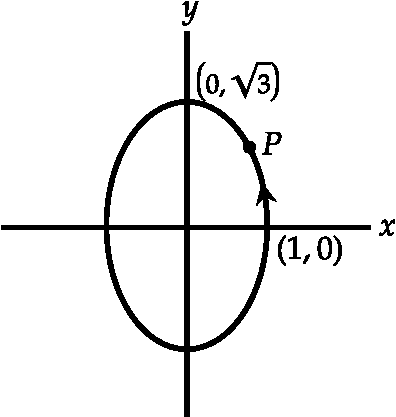
\includegraphics[height=4.5cm,width=4cm]{VI-Assignment-17}
	\end{figure}
	\begin{align*}
	\frac{x^{2}}{1}+\frac{y^{2}}{3}&=1
	\intertext{Point on ellipse is represented as}
	(\cos \theta, \sqrt{3} \sin \theta)&\\
	 \int \vec{F} \cdot d \vec{r} &=\int\left(\frac{x}{y} \hat{i}+\frac{y}{x} \hat{j}\right) \cdot(d x \hat{i}+d y \hat{j}) \\ &=\int \frac{x}{y} d x+\frac{y}{x} d y \\ &=\int_{0}^{\theta} \frac{\cos \theta}{\sqrt{3} \sin \theta}(-\sin \theta) d \theta+\frac{\sqrt{3} \sin \theta}{\cos \theta} \cdot \sqrt{3} \cos \theta d \theta \\ &=\int_{0}^{\theta}\left(-\frac{1}{\sqrt{3}} \cos \theta+3 \sin \theta\right) d \theta \\ &=-\frac{1}{\sqrt{3}} \sin \theta-\left.3 \cos \theta\right|_{0} ^{\theta} \\ &=-\frac{1}{\sqrt{3}} \sin \theta-3 \cos \theta+3 
	 \intertext{Work done in equal to 1}
	 \mathrm{So},&-\frac{1}{\sqrt{3}} \sin \theta-3 \cos \theta+3=1\\
	 \Rightarrow &\quad \frac{1}{\sqrt{3}} \sin \theta+3 \cos \theta=2\\
	 \Rightarrow &\quad\left(\frac{1}{\sqrt{3}} \sin \theta\right)^{2}=(2-3 \cos \theta)^{2}\\
	 \Rightarrow &\quad \frac{1}{3} \sin ^{2} \theta=4+9 \cos ^{2} \theta-12 \cos \theta\\
	 \Rightarrow &\quad 28 \cos ^{2} \theta-36 \cos \theta+11=0\\
	 \Rightarrow &\quad(2 \cos \theta-1)(14 \cos \theta-11)=0\\
	 \quad \cos \theta&=\frac{1}{2}, \frac{11}{14}
	 \intertext{So, there are two value of $\theta$ i.e., two possible location of $P$ such that the work done by $\vec{F}$ is 1 .}
	\end{align*}
\end{answer}
\item Find the circulation of the field
$$
\vec{F}=-x^{2} y \hat{i}+x y^{2} \hat{j}+\left(y^{3}-x^{3}\right) \hat{k}
$$
around the curve $C$, where $C$ is the intersection of the sphere $x^{2}+y^{2}+z^{2}=25$ and the plane $z=3$. The orientation of the curve $C$ is counterclockwise when viewed from above.
\begin{answer}$\left. \right. $
	\begin{figure}[H]
		\centering
		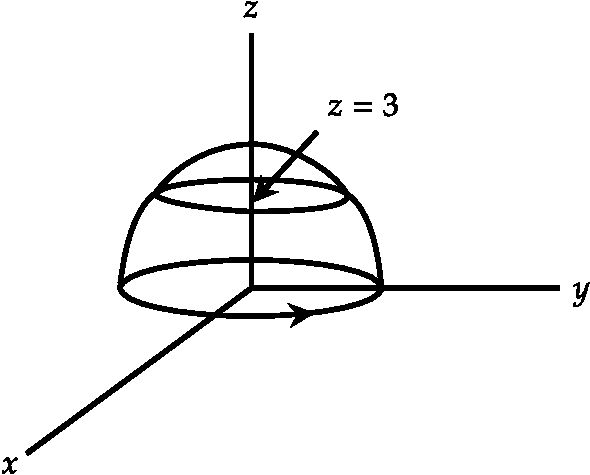
\includegraphics[height=4cm,width=5.2cm]{VI-Assignment-18}
	\end{figure}
	\begin{align*}
	\vec{F}&=-x^{2} y \hat{i}+x y^{2} \hat{j}+\left(y^{3}-x^{3}\right) \hat{k}
\intertext{	$C$ is the curve of intersection of surfaces}
	x^{2}+y^{2}+z^{2}&=25, z=3\\
	\text{So, }\quad x^{2}+y^{2}&=16\\
	\vec{F} \cdot d \vec{r}&=x^{2} y d x+x y^{2} d y+\left(y^{3}-x^{3}\right) d z\\
	\text{For curve }C, z&=3, d z=0\\
	\oint \vec{F} \cdot d \vec{r}&=\int-x^{2} y d x+x y^{2} d y\\
	\text{Let }x&=4 \cos \theta, y=4 \sin \theta\\
	 \oint \vec{F} \cdot d \vec{r} &=\int_{0}^{2 \pi}\left(256 \cos ^{2} \theta \sin ^{2} \theta d \theta+256 \cos ^{2} \theta \sin ^{2} \theta\right) d \theta \\ &=512 \int_{0}^{2 \pi} \sin ^{2} \theta \cos ^{2} \theta d \theta \\ &=512 \times 4 \int_{0}^{\pi / 2} \sin ^{2} \theta \cos ^{2} \theta d \theta \\ &=2048 \frac{\sqrt{3 / 2} \sqrt{3 / 2}}{2 \sqrt{3}}=128 \pi 
	\end{align*}
\end{answer}
\item If $\phi=2 x^{2} y z, \vec{F}=x y \hat{i}-z^{2} y \hat{j}+x^{2} \hat{k}$ and $C$ is the curve $x=2 t, y=t^{2}, z=t^{3}$ from $t=0$ and $t=1$. Evaluate the line integrals (a) $\int_{C} \phi d \vec{r}$ (b) $\int_{C} \vec{F} \times d \vec{r}$.
\begin{answer}
	\begin{align*}
\text{	(a)\quad Along }C, \phi&=2 x^{2} y z=2(2 t)^{2} \cdot t^{2} \cdot t^{3}=8 t^{7}\\
	\vec{r} &=x \hat{i}+y \hat{j}+z \hat{k} \\
	&=2 t \hat{i}+t^{2} \hat{j}+t^{3} \hat{k} \\
	d \vec{r} &=\left(2 \hat{i}+2 \hat{j}+3 t^{2} \hat{k}\right) d t \\
	\int_{C} \phi d \vec{r} &=\int_{0}^{1} 8 t^{7}\left(2 \hat{i}+2 t \hat{j}+3 t^{2} \hat{k}\right) d t \\
	&=\hat{i}_{0}^{1} 16 t^{7} d t+\hat{j}_{0}^{1} 16 t^{8} d t+\hat{k} \int_{0}^{1} 24 t^{9} d t \\
	&=2 \hat{i}+\frac{16}{9} \hat{j}+\frac{12}{5} \hat{k}\\\\
	\text{(b)\quad Along }C, \vec{F}&=x y \hat{i}-z^{2} y \hat{j}+x^{2} \hat{k}\\
	&=2 t^{3} \hat{i}-t^{8} \hat{j}+4 t^{2} \hat{k} \\
	\vec{F} \times d \vec{r} &=\left(2 t^{3} \hat{i}-t^{8} \hat{j}+4 t^{2} \hat{k}\right) \times\left(2 \hat{i}+2 t \hat{j}+3 t^{2} \hat{k}\right) \\
	&=\left|\begin{array}{ccc}
	\hat{i} & \hat{j} & \hat{k} \\
	2 t^{3} & -t^{8} & 4 t^{2} \\
	2 & 2 t & 3 t^{2}
	\end{array}\right| \\
	&=\left(-3 t^{10}-8 t^{3}\right) \hat{i}+\left(8 t^{2}-6 t^{5}\right) \hat{j}+\left(4 t^{4}+2 t^{8}\right) \hat{k} \\
	\int_{C} \vec{F} \times d \vec{r} &=\hat{i}_{0}^{1}\left(-3 t^{10}-8 t^{3}\right) d t+\hat{j} \int_{0}^{1}\left(8 t^{2}-6 t^{5}\right) d t+\hat{k} \int_{0}^{1}\left(4 t^{4}+2 t^{8}\right) d t \\
	&=-\frac{47}{11} \hat{i}+\frac{5}{3} \hat{j}+\frac{46}{45} \hat{k}
	\end{align*}
\end{answer}
\item Find the work done in moving the particle once round the ellipse $\frac{x^{2}}{25}+\frac{y^{2}}{16}=1, z=0$ under the field of force given by $\vec{F}=(2 x+y+z) \hat{i}+\left(x+y-z^{2}\right) \hat{j}+(3 x-2 y+4 z) \hat{k}$.
\begin{answer}
		Work done moving the particle by distance $d r$
		\begin{figure}[H]
			\centering
			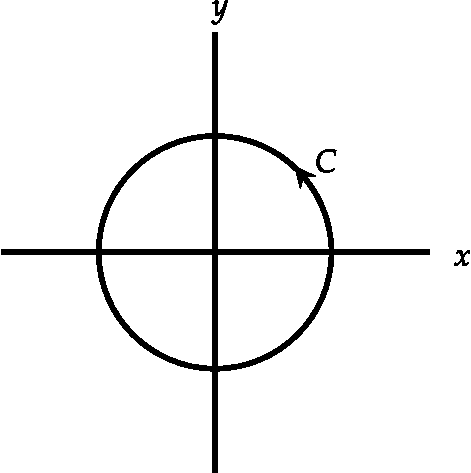
\includegraphics[height=3.5cm,width=3.5cm]{VI-Assignment-19}
		\end{figure}
	\begin{align*}
	\vec{F} \cdot d \vec{r}&=(2 x+y+z) d x+\left(x+y-z^{2}\right) d y+(3 x-2 y+4 z) d z\\
	\text{The curve $C$ is ellipse }&\frac{x^{2}}{25}+\frac{y^{2}}{16}=1\\
\text{	The equation  }&\text{of ellipse is given by}x=5 \cos \theta, y=4 \sin \theta, z=0\\
d x &=-5 \sin \theta d \theta \\ d y &=4 \cos \theta d \theta \\ d z &=0 \\ \vec{F} \cdot d \vec{r} &=(10 \cos \theta+4 \sin \theta)(-5 \sin \theta) d \theta+(5 \cos \theta+4 \sin \theta) 4 \cos \theta d \theta \\ &=\left(-34 \sin \theta \cos \theta+20 \cos ^{2} \theta-20 \sin ^{2} \theta\right) d \theta 
\intertext{On $C, \theta$ varies from 0 to $2 \pi$}
\intertext{So, work done in moving a particle around the ellipse}
\text{So, }\quad W&=\oint \vec{F} \cdot d \vec{r}\\
&=\int_{0}^{2 \pi}\left(-34 \sin \theta \cos \theta+20 \cos ^{2} \theta-20 \sin ^{2} \theta\right) d \theta\\
&=-34 \int_{0}^{2 \pi} \sin \theta \cos \theta d \theta+20 \int_{0}^{2 \pi} \cos ^{2} \theta d \theta-20 \int_{0}^{2 \pi} \sin ^{2} \theta d \theta \\
&=0
	\end{align*}
\end{answer}
\item Evaluate $\int_{C} \vec{F} \cdot d \vec{r}$ where $\vec{F}=c\left[-3 a \sin ^{2} \theta \cos \theta \hat{i}+a\left(2 \sin \theta-3 \sin ^{2} \theta\right) \hat{j}+b \sin 2 \theta \hat{k}\right]$ and the curve $C$ is given by $\vec{r}=a \cos \theta \hat{i}+a \sin \theta \hat{j}+b \theta \hat{k}, \theta$ varying from $\frac{\pi}{4}$ to $\frac{\pi}{2}$.
\begin{answer}
	\begin{align*}
	 \vec{r} &=a \cos \theta \hat{i}+a \sin \theta \hat{j}+b \theta \hat{k} \\ d \vec{r} &=(-a \sin \theta \hat{i}+a \cos \theta \hat{j}+b \hat{k}) d \theta \\ \vec{F} \cdot d \vec{r} &=c\left[3 a^{2} \sin ^{3} \theta \cos \theta+a^{2}\left(2 \sin \theta-3 \sin ^{2} \theta\right) \cos \theta+b^{2} \sin 2 \theta\right] d \theta 
	 \intertext{The line integral}
	  \int_{C} \vec{F} \cdot d \vec{r} &=3 a^{2} c \int_{\pi / 4}^{\pi / 2} \sin ^{3} \theta \cos \theta d \theta+a^{2} c \int_{\pi / 4}^{\pi / 2}\left(2 \sin \theta-3 \sin ^{2} \theta\right) \cos \theta d \theta+b^{2} c \int_{\pi / 4}^{\pi / 2} \sin 2 \theta d \theta \\ &=3 a^{2} c\left[\frac{\sin ^{4} \theta}{4}\right]_{\pi / 4}^{\pi / 2}+a^{2} c\left[\sin ^{2} \theta-\sin ^{3} \theta\right]_{\pi / 4}^{\pi / 2}-\frac{b^{2} c}{2}[\cos 2 \theta]_{\pi / 4}^{\pi / 2} \\ &=\frac{9}{16} a^{2} c+a^{2} c\left[\frac{1}{2}-\frac{1}{2 \sqrt{2}}\right]+\frac{b^{2} c}{2} \\ &=\left(\frac{17}{16}-\frac{1}{2 \sqrt{2}}\right) a^{2} c+\frac{b^{2} c}{2} 
	\end{align*}
\end{answer}
\end{enumerate}
\section{Green's Theorem}
\begin{enumerate}
	\item Verify Green's theorem in the place for $\oint_{C}\left(x y+x^{2}\right) d x+x^{2} d y$ where $C$ is the closed curve of the region 
	bounded by $y=x$ and $x^{2}=4 a y$.
	\begin{figure}[H]
		\centering
		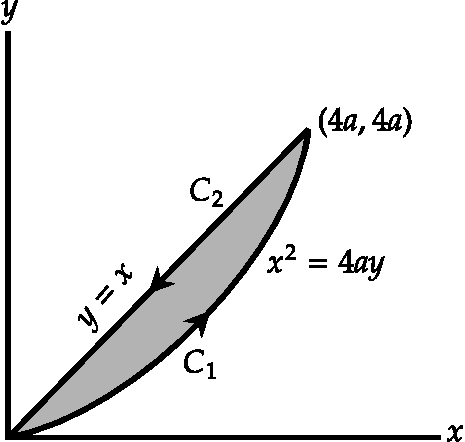
\includegraphics[height=4cm,width=4.5cm]{GT-Assignment-01}
	\end{figure}
	\begin{answer}
		\begin{align*}
	\text{	Here }M d x&+N d y\\
		&=\left(x y+x^{2}\right) d x+x^{2} d y \\
		M&=x y+x^{2} \Rightarrow \frac{\partial M}{\partial y}=x \\
		N&=x^{2} \quad \Rightarrow \frac{\partial N}{\partial x}=2 x
		\intertext{Let us first evaluate the double integral over Region $R$ bounded by $x^{2}=4 a y$ (curve $\left.C_{1}\right) \& y=x$ (curve $C_{2}$ ) as}
	 \iint\left(\frac{\partial N}{\partial x}-\frac{\partial M}{\partial y}\right) d x d y &=\int_{0}^{4 a} \int_{x^{2} / 4 a}^{x} x d y d x \\ &=\int_{0}^{4 a} x\left(x-\frac{x^{2}}{4 a}\right) d x=\frac{x^{3}}{3}-\left.\frac{x^{4}}{16 a}\right|_{0} ^{4 a}=\frac{16 a^{3}}{3} 
	 \intertext{Now let us evaluate the line integral $\oint M d x+N d y$ on closed curve $C$. The curve $C$ is a piecewise smooth curve consisting of $C_{1}$ and $C_{2}$.}
	\text{ On }C_{1}, y&=\frac{x^{2}}{4 a}\quad 
	 d y=\frac{x}{2 a} d x\\
	 M d x+N d y &=\left(x y+x^{2}\right) d x+x^{2} d y \\ &=\left(\frac{x^{3}}{4 a}+x^{2}\right) d x+x^{2} \frac{x}{2 a} d x \\ &=\left(\frac{3}{4} \cdot \frac{x^{3}}{a}+x^{2}\right) d x 
	 \intertext{$x$ varies from 0 to $4 a$ on $C_{1}$}
	\text{ So,}
	 \int_{C_{1}} M d x+N d y&=\int_{0}^{4 a}\left(\frac{3 x^{3}}{4 a}+x^{2}\right) d x\\
	 &=\frac{3}{16 a} x^{4}+\left.\frac{x^{3}}{3}\right|_{0} ^{4 a}\\
	 &=8 a^{3}+\frac{64 a^{3}}{3}=\frac{208 a^{3}}{3}\\
	 \text{On }C_{2}, \quad y&=x, d y=d x\\
	 M d x+N d y &=\left(x y+x^{2}\right) d x+x^{2} d y \\ &=3 x^{2} d x 
	 \intertext{$x$ varies from $4 a$ to 0 .}
	\text{ So,}
	 \int_{C_{2}} M d x+N d y&=\int_{4 a}^{0} 3 x^{2} d x\\
	 &=\left.x^{3}\right|_{4 a} ^{0}=-64 a^{3}\\
	  \text{so, }\int_{C} M d x+N d y &=\int_{C_{1}} M d x+N d y+\int_{C_{2}} M d x+N d y \\ &=\frac{208}{3} a^{3}-64 a^{3}=\frac{16}{3} a^{3} \\
	 \text{ Since, }
	  \iint_{R}\left(\frac{\partial N}{\partial x}-\frac{\partial M}{\partial y}\right) d x d y&=\oint_{C} M d x+N d y
	 \intertext{ So, Green's theorem is verified.}
		\end{align*}
	\end{answer}
	\item 	Apply Green's theorem in the plane to evaluate $\oint\{(y-\sin x) d x+\cos x d y\}$ where $C$ is the triangle enclosed by the lines $y=0, x=\pi, \pi y=2 x$.
	\begin{answer}$\left. \right. $
		\begin{figure}[H]
			\centering
			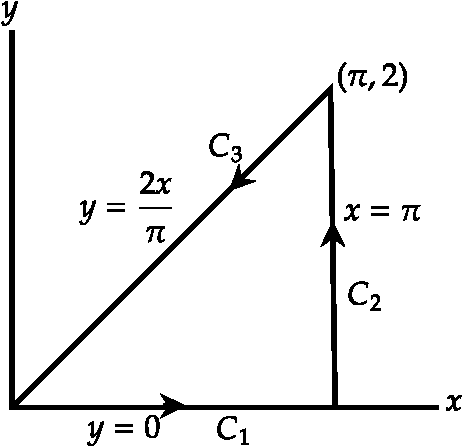
\includegraphics[height=4cm,width=4cm]{GT-Assignment-06}
		\end{figure}
		\begin{align*}
	\text{	Here, }\quad M d x+N d y&=(y-\sin x) d x+\cos x d y\\
	\text{So, }\quad M&=y-\sin x, \quad \frac{\partial M}{\partial y}=1\\
	N&=\cos x, \quad \frac{\partial N}{\partial x}=-\sin x
	\intertext{According to Green's theorem}
	\oint_{C} M d x+N d y&=\iint_{R}\left(\frac{\partial N}{\partial x}-\frac{\partial M}{\partial y}\right) d x d y
	\intertext{where $R$ is the region enclosed by the piecewise smooth curve $C$ consisting of curve $C_{1}(y=0)$, curve $C_{2}(x=\pi)$ curve $C_{3}(\pi y=2 x)$ as shown in Figure 9.4.}
	\text{So, }\quad \iint\left(\frac{\partial N}{\partial x}-\frac{\partial M}{\partial y}\right) d x d y&=\int_{0}^{2} \int_{\pi y / 2}^{\pi}(-\sin x-1) d x d y\\
	&=\int_{0}^{2}[\cos x-x]_{\pi y / 2}^{\pi} d y\\
	&=\int_{0}^{2}\left(-1-\pi-\cos \frac{\pi y}{2}+\frac{\pi y}{2}\right) d y\\
	&=-(1+\pi) y-\frac{2}{\pi} \sin \frac{\pi y}{2}+\left.\frac{\pi y^{2}}{4}\right|_{0} ^{2}=-2-\pi
		\end{align*}
	\end{answer}
	\item If $\vec{F}=\left(x^{2}-y^{2}\right) \hat{i}+2 x y \hat{j}$ and $\vec{r}=x \hat{i}+y \hat{j}$, find the value of $\oint\left(x^{2}-y^{2}\right) d x+2 x y d y$ around the rectangular boundary $x=0, x=a, y=0$ and $y=b$.
	\begin{answer}
		Here, the curve $C$ is a piecewise smooth curve consisting of $C_{1}(y=0), C_{2}(x=a), C_{3}(y=b) \& C_{4}$ $(x=0)$.\\
		The region bounded by $C$ is shown in figure $9.5$.
		\begin{figure}[H]
			\centering
			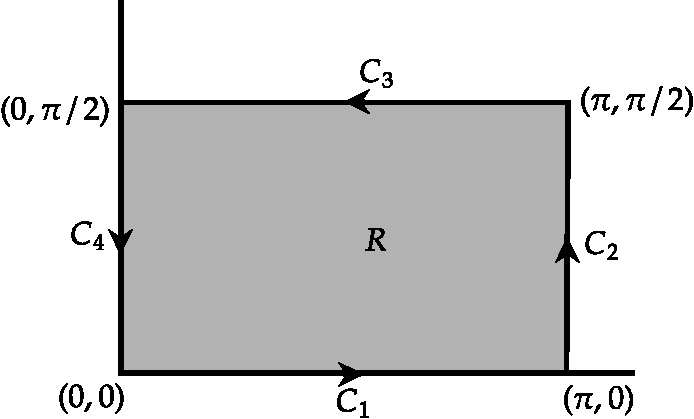
\includegraphics[height=3cm,width=5cm]{GT-Assignment-02}
		\end{figure}
		\begin{align*}
		\oint \vec{F} \cdot d \vec{r}&=\oint\left(x^{2}-y^{2}\right) d x+2 x y d y=\oint M d x+N d y\\
		\text{Here, }M&=x^{2}-y^{2}, \quad \frac{\partial M}{\partial y}=-2 y\\
		N&=2 x y, \quad \frac{\partial N}{\partial x}=2 y
		\intertext{Applying Green's theorem}
		 \oint M d x+N d y &=\iint\left(\frac{\partial N}{\partial x}-\frac{\partial M}{\partial y}\right) d x d y \\ &=4 \int_{0}^{b} \int_{0}^{a} y d x d y=4 a \int_{0}^{b} y d y \\ &=2 a b^{2} 
		\end{align*}
	\end{answer}
	
	
	
	
	
	
	
	
	
	
	
	
	
	
	
	
	
	
	
	
	
	
	
	
	
	
	
\end{enumerate}